

\documentclass[12pt]{article}
\usepackage[utf8]{inputenc}
\usepackage{graphicx}
\usepackage{subfig}
\usepackage{url}
\usepackage{xcolor}
\usepackage{comment}
\usepackage{mathptmx} % Times New Roman font
\usepackage{geometry} % margins
\usepackage{authblk} % affiliations
\usepackage{indentfirst} % indent first paragraph
\usepackage{amsmath}
\usepackage{amsfonts}
\usepackage{amssymb}
\usepackage{caption}
\captionsetup[table]{position=bottom}   %% or below
\usepackage{hyperref}
%next two packages allows table to float within text
\usepackage{float}
\usepackage[super]{nth}
\restylefloat{table}
\usepackage{enumitem} %to make lists
\setlist[description]{leftmargin=\parindent,labelindent=\parindent}


%%%%%%%%%%%%%%%%%%%%%%%%%%%%%%%%%%%%%%%%%%%
% Page Setup
\pagenumbering{gobble}
\geometry{margin=1in}

% separation between title/authors/affiliations
\setlength{\affilsep}{1.5em}
% make paragraph indent larger
\setlength{\parindent}{3.5em}

%Sets the size of the affiliations to that of footnotes
\renewcommand\Affilfont{\footnotesize}
\makeatletter
 \def\@maketitle{%
   \newpage
   \begin{center}%
   \let \footnote \thanks
     {\huge\bfseries \@title \par}%
     \vskip \@affilsep%
     {\large%
         \begin{tabular}[t]{c}%
         \@author\\
         contact: \href{mailto:\contact}{\contact}
       \end{tabular}\par}%
   \end{center}}
 \makeatother
 
 
%end Page Setup
%%%%%%%%%%%%%%%%%%%%%%%%%%%%%%%%%%%%%%%%%%%
%Title & Affiliation Settings
\title{From Zipf's Law to Power Laws: Is Conversational Speech Zipfian?}
\def\contact{jkilfoyle@unm.edu}
\author[1]{Jeb Kilfoyle}
\author[2]{Paul De Palma}
\author[2]{Phillip Fishburn}
\author[2]{Alex Giacobbi}
\author[2] {Leon Garcia-Carmargo}
\author[3]{Joseph Stover}
\author[4]{Mark VanDam}
\affil[1]{Department of Computer Science, University of New Mexico}
\affil[2]{Department of Computer Science, Gonzaga University}
\affil[3]{Department of Mathematics, Gonzaga University}
\affil[4]{Department of Speech and Hearing Sciences, Washington State University}
%%%%%%%%%%%%%%%%%%%%%%%%%%%%%%%%%%%%%%%%%%%

\begin{document}

\maketitle  %Generate title and the affiliations
\section*{\centering\large Abstract}
\noindent Zipf's law describes the relationship between the frequency of words in a large corpus and their rank.  Its most basic form is a harmonic series, indicating that the frequency of words is inversely proportional to rank.  The past two decades have seen the emergence of usage-based and cognitive approaches to language study.  A key observation of these approaches is that speech differs in substantial and structural ways from writing.  Except for a few older analyses performed on very small corpora, all studies of Zipf's law have been done on written corpora.  Our primary research question is this: "Do the words which comprise transcribed speech corpora follow a Zipfian distribution?"  This paper examines several transcribed speech corpora to see if spoken words form a Zipfian distribution.  In addition, many presentations of Zipf's law use informal methods to determine whether a given distribution is Zipfian.  A log-log plot of frequency against rank with slope of approximating -1 is frequently enough for the distribution to be judged Zipfian.  This paper uses the Kolmogorov-Smirnov statistic in conjunction with more rigorous and recently developed statistical techniques to judge whether a corpus under examination is Zipfian. Speech, in the corpora examined, is shown to be Zipfian.\\

\noindent Acknowledgements: The authors would like to thank Robert and Claire McDonald and the McDonald Work-Award Program for their generous and continuous support for undergraduate research assistants.  They would also like to thank former students, Bethany Bogensberger and Allison Hayes, who contributed to earlier versions of this work. 

\section{Introduction}

The title of this article is posed as a question, but implies answers to two preceding questions, each with an embedded prior question: 1) What is meant by "conversation," (and why do we care about it); and 2) What is meant by "Zipfian" (and how do we know it when we see it).  Since we have framed question 1 by its modifier, "Zipfian,"  in question 2, the paper begins with a discussion of "Zipfianness" in the first two sections.   We discuss conversation in Section 3.  Section 4 applies rigorous and recently developed statistical techniques to the question of whether conversation is Zipfian.  Section 5 discusses some implications of the research presented here and suggests possible future directions.  

Any student of linguistics can confidently recite Zipf's Law: the frequency of a word in a language is inversely proportional to its rank.  More precisely, the second ranked word is half as frequent as the first, the third is one-third as frequent as the first, and so on:
\begin{center}
\[\frac{1}{2}, \frac{1}{3}, \frac{1}{4},...\]
\end{center}

It is a remarkable result, usually attributed to George Kingsley Zipf, a Harvard philologist, whose 1949 book, \emph {Human Behavior and the Principle of Least Effort} (Zipf, 1949), manages to sound contemporary and quaint at the same time: "Nearly twenty-five years ago, it occurred to me that we might gain considerable insight into the mainsprings of human behavior if we viewed it purely as a natural phenomenon like everything else in the universe, and if we studied it with the same dispassionate objectivity with which one is wont to study, say, the social behavior of bees, or the nestbuilding habits of birds" (Zipf, 1949, p. v).\footnote[1]{Newman (2005) says pride of first place actually belongs to the German physicist, Felix Auerbach, who observed in 1913 that city populations are inversely proportional to their rank.  Newman seems not have noticed two previous studies that Zipf undertook, published in 1929 and 1932.  These are formulations of what has come to be called Zipf's Law, but with respect to phonetics and phonology instead of word count.  Said Zipf in 1929, "...the conspicuousness or intensity of any element of language is inversely proportionate to its frequency" (pp. 88-89).  In both monographs Zipf was attempting to account for language change, though in the second, he was engaged in cross-linguistic study, comparing "the modern vernacular of Peking, China" with his findings from 1929 for "Indo-European tongues" (Zipf, 1932, p. 1). In a world without Google Scholar, it is not surprising that he does not cite Auerbach's German paper, though he himself was an "Instructor in German," according to the frontispiece of his 1932 article. The Zipf/Auerbach story seems yet another instance of co-discovery, common in science.}  Relying on a previously published (1937) and hand-counted indices of words and their frequencies in James Joyce's \emph{Ulysses} (Hanley, 1937/1962), and a sample of American newspapers, he produced the familiar log-log plot for word frequency against rank along with the idealized line whose slope is -1, which is found in modern papers on Zipf's law.  See, for example Ha, \emph{et al. (2002)}. \\
\indent As it happens, word frequencies are not the only phenomenon that are distributed according to the rule that we will call (for now), "Zipf's Law."  Magnitudes of earthquakes, intensities of solar flares, citations of scientific papers, web hits, wealth, family names, and city populations all appear to follow a Zipfian distribution (Newman, 2005).  What these phenomenon have in common is intuitively obvious.  There are very few of each with high numbers (rich people, large earthquakes, heavily cited papers, etc.), and a great many with low numbers (poor people, small earthquakes, rarely cited papers, etc.).   Figure 1a is a plot of the rank order of the world's richest people against their wealth.  Figure 1b is, with a nod to Zipf's classic example, a plot of the rank order of words in James Joyce's \emph{Ulysses} against their frequencies .   

\begin{figure}[h!]
    \centering
    \subfloat[Rank against Wealth]{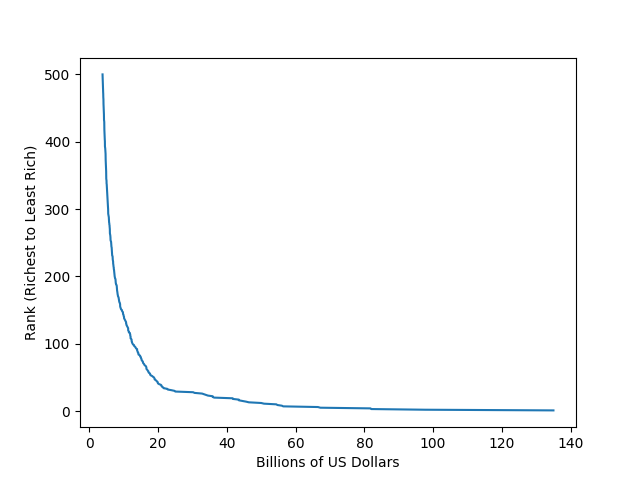
\includegraphics[width=0.4\textwidth]{wealth.png}\label{fig:f1}}
    \hfill
    \subfloat[Rank against Word Frequency]{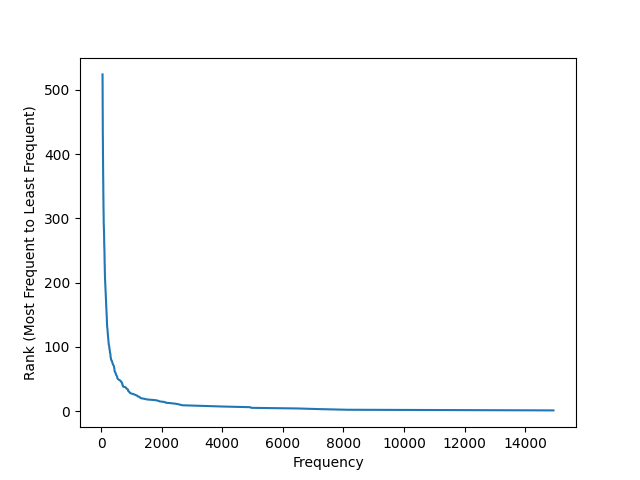
\includegraphics[width=0.4\textwidth]{ulyssesRXF.png}\label{fig:f1}}
    \caption{Wealth and Words}%
\end{figure}
Both plots tell the same story.  Here is the story for wealth:  although all five hundred of the world's richest people may well be rich, a very few are the richest of all (\emph{Bloomberg Billionaire's Index}, 2020).  The story of words is similar. The plots can seem mysterious. What, beyond intuition, does wealth have to do with words?  Where does the distinctive shape come from? Is there a closed form formula beyond the basic inverse relationship between frequency and rank that produces both plots (and those of wildly disparate phenomena)?  Mathematical treatments of Zipf's Law in the literature tend to be forbiddingly formal, stated without explanation, or so simple as to miss its richness.  See, for example Baayen (2001), Cancho (2005), Ridley (1994).   The next section is (we hope) a readable, yet rigorous, treatment of the origins of Zipf's Law.  It is intended to fill a gap in word distribution studies.  After that, we turn to a very short discussion of some of the most important differences between the writing and conversation.  At that point we will turn our attention to the primary concern of this paper, the application of relatively new statistical techniques to analyze whether the words in conversation form a Zipfian distribution.


\section{Where Does Zipf's Law Come From?}

\indent 
Perhaps the easiest way to begin a discussion of Zipf's Law is to begin with Zipf himself.  Early on in his 1949 book, he presents a formula derived from observing word frequencies in James Joyce's \emph{Ulysses}. Zipf used the Hanley index\footnote[2]{To learn how the index was created is to be simultaneously inspired by human ingenuity and profoundly grateful for computing.} to the book, originally published in 1937  (Hanley, 1937/1962).  To illustrate Zipf's findings, we have downloaded and tokenized the version of \emph{Ulysses} available from Project Gutenberg (Project Gutenberg, 2020).  Let \emph{f} be the frequency of occurrence of a word in a text, and \emph{r} the rank of that word.  Then the products of words and ranks are approximately the same.  Zipf expresses this in Eq. (1).  

\begin{align}
r\times f = C
\end{align}

Table 1 is our version of Zipf's presentation of selected ranks and frequencies. The ranks shown were chosen by Zipf, though his lowest rank was 29,899 reflecting more word types generated by Hanley's tokenization algorithm than by our own.\footnote[3]{The numbers in Table 1 differ slightly from Zipf's, due most likely to differences in editions and tokenization technique.  The inferences licensed by the numbers are the same as Zipf's, however, which will become clear as we proceed.  We initially used \emph{word\_tokenize} from the Natural Language Tool Kit to separate the text into words, but found that we got better results, i.e., closer to Hanley's, if we split sequences of characters on spaces and line breaks.  We then removed punctuation and digits.   As in Hanley, each word form (e.g., "give," "given") is a separate word (Hanley, 1937/1962; NLTK, 2020).}  

\begin{table}
\begin{center}
 \begin{tabular}{||l l l|| }
 \hline
 Rank &  Freq  & $C$ \\
 \hline
    10 & 2606& 26060    \\
    20 & 1319 & 26380   \\
    30 & 934 & 28020    \\
    40 & 719 & 28760    \\
    50 & 554 & 27700    \\
    100 & 272 & 27200   \\
    500 & 52 & 26000    \\
    1000 & 26 & 26000   \\
    2000 & 12 & 24000   \\
    3000 & 8 & 24000    \\
    4000 & 6 & 24000    \\
    5000 & 5 & 25000    \\
    10000 & 2 & 20000   \\
    20000 & 1 & 20000   \\
    29477 & 1 & 29477   \\
  \hline
\end{tabular} 
\caption{Word Ranks, Frequencies, and their Products (\emph{C}) from James Joyce's \emph{Ulysses}}
\end{center}
\end{table}
Zipf makes much of the third column, "which is approximately the same for all the different ranks" (Zipf, 1949, p. 23), though he never defines "approximately."  The floor of the standard deviation of this column for all ranks is 3,894.  If we omit words used ten times or fewer, the standard deviation drops to 1,110.\footnote[4]{Theresa Fein, Hanley's assistant, noted that the pattern is clearer if the extremes are omitted, though, without a computer to easily test her hypothesis, she recommended in 1937 dropping "the few dozen most frequent words" and those "that occur only once or twice" (Hanley, 1937/1962, p. 386)}  
"Approximately" seems appropriate, especially with the outliers removed. 

The computation of rank times frequency led Zipf to another observation that is not often mentioned in the literature on Zipfian distributions.  This is $r \times f$ times a text-specific constant yields an approximation of the size of the text itself. The constant Zipf discovered in the case of \emph{Ulysses} is 10.  If we multiply the values in the third column, both with and without the word groups noted above, the approximations are 223,674 and 258,172, respectively.   The number of tokens in the Project Gutenberg edition of \emph{Ulysses} is 262,799, a reasonable approximation, especially since no one before Zipf had noticed the relationship.   What we are really talking about here are that words in a text, wealth in a population, or any number of other phenomena organize themselves in such a way that their probabilities cause Figures 1a and 1b to be generated. 

Since $r\times f = C$, and, of course, $f = \frac{C}{r}$, then, with $N$ the number of words in the text and $C$ the proportionality constant, word frequencies decrease in proportion to a simple harmonic series:


\begin{align}
1,\frac{1}{2},\frac{1}{3},\frac{1}{4},...\frac{1}{\emph{N}}
\end{align}
\noindent

With a few adjustments, this series of ratios can be reformulated as a series of probabilities. Suppose for a given text, $w_r$ is the word of rank $r$, $f_r$ is the frequency of $w_r$, and $p_r$ is the probability of word $w_r$ occurring in the text, then,
\begin{align}
p_r=\frac{f_r}{N}=\frac{C}{r}\times\frac{1}{N}
\end{align}
\noindent
Let $\frac{C}{N} = C_1$.  Then, for every group of words associated with a distinct rank, the probability of each word in the group is $p_r = \frac{C_1}{r}$.  This gives us a harmonic series as above, but with a different proportionality constant, $C_1$. This time, however, it is also a normalizing constant whose task is to ensure that the probabilities sum to 1:
\begin{align}
\sum_{r=1}^{n} p_r = 1
\end{align}
\noindent
Here $n$ is the rank of the least frequent word, and $p_r$ is the probability that word $w_r$ would be chosen from a random sample.  

Figure 1b plots word rank against word frequency for the 524 words in \emph{Ulysses} that appear at least fifty times.\footnote[5]{This reverses Zipf's X and Y axes in his 1949 book, though not in the 1929 or 1932 monographs.  Both orderings produce the same graph, though flipped for a log-log plot. Using frequency as the independent variable makes the the derivation of the closed-form formula clearer.  In Section 3, we use Zipf's ordering to be consistent with his work. The \nth{525} most frequent word, \emph{neck}, occurs forty-nine times. Restricting the display to types occurring less than fifty times makes a cleaner plot, but does not change the argument being made or the numbers in Table 1.}  We are looking for the closed form formula for the function, call it $R$, that produces the plot.  First, notice the probabilities of the five most frequent words in \emph{Ulysses}, shown in Table 2.  

\begin{table}[h!]
\begin{center}
 \begin{tabular}{||l l l||}
 \hline
 Word &  Frequency  & Probability \\
 \hline
    the & 14934& 0.0568    \\
    of & 8141 & 0.0310   \\
    and & 7214 & 0.0274    \\
    a & 6502 & 0.0247    \\
    to & 4959 & 0.0189    \\
  \hline
\end{tabular} 
\caption{Five Most Frequent Words in James Joyce's \emph{Ulysses}}
\end{center}
\end{table}

The sum of probabilities over all word ranks is 1, just as the sum of the frequencies over all words is $N$, the total number words in the text.  Since \emph{the} is the most frequent word, its probability is greater than or equal to the probability of any other word.  Said another way, there is exactly one word, namely \emph{the}, with a probability equal to or greater than \emph{the}.  An analogous relationship holds for the second most frequent word, \emph{of}: there are exactly two words with probability greater than or equal to that of \emph{of}.  In fact, there are exactly \emph{q} words with probability greater than or equal to the probability of the \emph{qth} most frequent word, and, of course, the \emph{qth} most frequent word is the word of rank \emph{q}.  Notice we are using the words \emph{frequency} and \emph{probability} almost interchangeably.  This is because probability is just frequency normalized by $N$, the number of words in the text as shown in Eq.(3).   This means that plot of ranks against probabilities looks the same as a plot of ranks against frequencies.  Figure 2, except for the X scale and both legends, is identical to Figure 1b.  

\begin{figure}[h!]
    \centering
    \includegraphics[width=0.4\textwidth]{ulyssesRXP.png}\\
    \caption{Word Rank against Word Probability}%
\end{figure}

Notice as we move up on the Y axis, the probability of the use of the word decreases sharply.  As we move right on the X axis, the probability that a word will be used increases along with its rank, which, of course, is in reverse order of its frequency.  Imagine a very small interval on the X axis just to the right of some probability, $p$.  Call this interval $dp$.  Since $R(p)$ is the height on the Y axis, $R(p)\; x\; dp$ is the area of an infintessimally slender rectangle.  If we performed this exercise and summed the products over all possible tiny rectangles, we would have a close approximation of the area under the plot, expressed as an integral in Eq.(5):

\begin{align}
\int_{0}^{0.0568} R(p)dp
\end{align}

$R$ is a cumulative distribution function, whether applied to frequencies, $f$, or probabilities, $p$.  It has the property that as you move along the X axis, in Figure 1b,  $R(f)$ gives the rank of the word whose frequency is greater than or equal to $f$.  Notice that the ranks themselves can be normalized by $N$.  Then, $R(f)$ is the fraction of words with frequency greater than or equal to $f$. 

We are now ready to develop a more general version of the relationship Zipf discovered empirically and expressed in Eq. (1).  When the natural log of word rank (or probability) is plotted against the natural log of word frequency, "a remarkable pattern emerges," words unusually expressive for a physics journal (Newman, 2005, p. 1).  Namely, Figure 2 (or Figure 1) becomes a nearly straight line with a negative slope as shown in Figure 3.  

\begin{figure}[h]
    \centering
    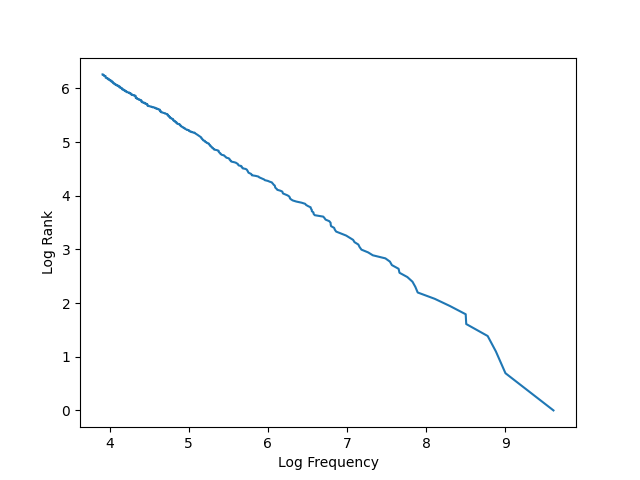
\includegraphics[width=.4\textwidth]{ulyssesLogRXF.png}\\
    \caption{Log Word Rank against Log Word Frequency}%
\end{figure}

Zipf noticed this as early as 1929, though suggesting in 1949 that it was mostly a useful way to present compactly the rank/frequency relationship for nearly thirty thousand word types.   The straight line on a double log plot, or rather its approximation, is the key to deriving a general closed-form formula for Zipf's law.  The point-slope formula for a straight line is, of course, $y = mx + b$ where $m$ is the slope of the line and $b$ is where it intercepts the vertical axis.  But since the line shown in Figure 3 plots log(y) against log(x) and has a negative slope, the equation that approximates it becomes:

\begin{align}
\log(y) = -m \cdot log(x) + b
\end{align}

\noindent Taking the exponential (or antilog) of Eq.(6) as in Eq.(7) gives Eq.(8):
\begin{align}
\exp(log(y) = exp(-m \cdot log(x) + b)
\end{align}

\begin{align}
y = x^{-m}exp(b) = x^{-m} \cdot e^b
\end{align}

Since $e^b$, is constant for a given line, we can replace it with $C$, giving:

\begin{align}
y = Cx^{-m}
\end{align}

\noindent Finally, to be consistent with the notation we have been using, as well as that which is common in the literature, we can rewrite Eq.(9) as:


\begin{align}
R(f) = Cf^{-\alpha}
\end{align}



\noindent This is the closed-form formula for Zipf's law, except in this more general form, it is usually referred to as a \emph{power law}.  If we take $\alpha$ to be 1, as Zipf did, then we have Eq.(1), which Zipf used to express the relationship he discovered empirically between word rank and word frequency in \emph{Ulysses} (Zipf, 1949).\footnote[6]{From this point in the paper, whenever we mention Zipf's Law or \emph{Zipfian} or \emph{Zipfianness}, we are talking talking about power law behavior as formulated in Eq.(10), unless we explicitly say otherwise. Newman (2005) provides a clear and complete treatment of power law distributions, along with the derivation shown here.  Baayen's book (2002) is a highly technical discussion of word frequency distributions and covers some of the same issues.}

Zipf's project over two decades was first, to discover the relationship of the harmonic series to word sequences and, then, to argue that it was for human language, a "standard curve of distribution."  Conformity to such a curve or deviation from it could "shed light on significant factors in the structure of language" (Zipf 1935, p.47, as quoted in Baayen, 2001, p.17).  Zipf was right, although things were more complicated than he thought.   Once computation arrived on the scene and larger corpora became available, it became clear that a slope of -1 in the log-log rank-frequency plot was only an approximation.  Researchers, like Herbert Simon (of early AI fame) and Benoit Mandelbrot (of the Mandelbrot Set), debated various modifications to Zipf's Law (Ha, 2002; Fedorowicz, 1982).  Nevertheless, Zipf's Law remains a special case of power law distributions, and, as we argue at the end of this paper, when accompanied by contemporary statistical analyses, may prove useful in diagnosing speech-disordered conditions (something Zipf himself pioneered in his examination of  "schizophrenic speech" (Zipf, 1949, p. 288).  This will require analyzing speech from a Zipfian perspective.  Though Zipf used spoken as well as written data from the start, he appeared to use them interchangeably.  We briefly address this in the next section. 


\section{Why Conversation Matters}
Something that strikes a contemporary linguist as curious in Zipf's work is the way in which he conflates conversational speech and writing.  Here, for example, is Zipf in 1949 introducing his work:
\begin{quote}
Since the number of different words in a sample of speech together with their respective frequencies of occurrences can be determined empirically, it is clear that our next step is to seek relevant empiric information about the number and frequency of occurrences of words in some actual samples of speech.
\end{quote}
So far so good.  Yet the very next sentence reads, "James Joyce's \emph{Ulysses}, with its 260,430 running words, represents a sizable sample of running speech that may be fairly said to have served successfully in the communication of ideas" (Zipf, 1949, p. 23).  One more among many possibilities should be sufficient to persuade that for Zipf the difference between speech and writing is purely an accident of differing media: "There is a 1 to 1 correspondence between spoken speech and written speech, even though sound is the physical medium of the one while light is the physical medium of the other" (Zipf, 1949, p. 272).  

This is a naive view of language, even naive for 1949 when it was published.  Milman Parry, a contemporary of Zipf's at Harvard, had published work on the distinctive oral structure of the Homeric epics, work that the rhetorician, Walter Ong, was to turn into a lifetime examination of the differences between speech and writing, beginning in the fifties with his magisterial study of the sixteenth century logician, Peter Ramus.   Even Leonard Bloomfield, also at Harvard and also at the same time, argued in 1935 that writing, far from being language, was simply a means of recording language (Parry, 1928/1971; Ong, 1958; Miller and Weinert, 1998).  

However, it was not until inexpensive recording and storage devices began to make large speech corpora possible that the structural differences between writing and spontaneous spoken speech began to become obvious.   Perhaps the best-known of these corpora are the Watergate tapes, where readers in the seventies were apparently surprised to find that very few spoken word strings correspond to what we might call a sentence.  There was structure, of course, what Tomasello (2003) calls "intonation units," yet structure of a very different kind than that generated by what we might call, a "grammar."  

Yet another difference is the immediacy and apparent simplicity of speech as opposed to writing.   Utterances in which an agent causes a change of state in another participant are less frequent in speech than in writing.  Some items, on the other hand, are more common in speech, for example, verbs spread across several lexical items, as in, "he \emph{went to all the trouble of cooking} a nice dinner." These differences and many, many others come from the distinctive way in which spontaneous spoken language is produced and heard. It is done in real-time, under the limitations of short-term memory, involving modulations in pitch, rhythm, amplitude, and accompanied by gestures, visual focus, and body position (Miller and Weinert, 1998).  

As Ong famously and presciently wrote in 1977 (p. 53), "The writer's audience is always a fiction." An elaborate set of syntactic and discourse-related devices are necessary to construct that fiction, to fill in for gestures, pitch, body position and all the rest.  These observations, crucially dependent upon the availability of inexpensive digital recording, storage, and computing devices have given rise to large sub-fields in language study, automatic speech recognition, for example, and aspects of cognitive, functional, and usage-based linguistics. It is not obvious that because written corpora are Zipfian to some degree of approximation, that the same should hold true for spoken language.



\section{Materials and Methods}
\subsection{Materials}
We now turn to the two primary goals of this paper: 1) To develop a test for Zipfianness more sophisticated than a simple visual or regression scan of a log-log plot and 2) To determine, using this test, whether several corpora of spoken language are Zipfian.   To do so we use:
\begin{itemize}
    \item The Python programming language (python.org) and matplotlib (matplotib.org) to tokenize some of the written corpora and to do the rank/frequency plots in Sections 1 and 2
    \item The R Project for Statistical Computing (r-project.org) to encode the techniques described in Subsections 4.1 and 4.2
    \item The corpora listed in Table 3, along with James Joyce's \emph{Ulysses} from Project Gutenberg (Project Gutenberg, 2020). 
\end{itemize}

\begin{table}[h!]
\begin{center}
 \begin{tabular}{||l l l || }
 \hline
 Corpus &  Type  & No. Words \\
 \hline
 Buckeye & SS & 277,795 \\ 
 Santa Barbara & SS & 234,259 \\
 MiCase & AS & 1,652,747 \\
 Czech & TS & 146,384 \\
 Fisher & TS & 6,838,332 \\ 
 ATIS   & RS & 151,415 \\
 Brown & W & 1,012,528 \\
\hline
\end{tabular}
\caption{Corpora}
\end{center}                                                                                                                                                                                                                                                                                                                                                                                                                                                                                  
\end{table}

The corpora differ in language mode and the circumstances of collection.  Brown is clearly a written corpus (W), in fact, famously the first million word corpus of written English. We provide it as a point of comparison with the spoken corpora.  Buckeye (Pitt \emph{et al.}, 2007) and Santa Barbara (Du Bois \emph{et al.} 2000-2005) are collections of spontanious speech.   MiCase (Simpson, \emph{et al.}, 2002) is also spontaneous speech, but in the academic register.  Since Miller and Weinert (1998) suggest that such speech has elements of written language, we will call this corpus \emph{academic speech}, AS.  Both Fisher (Cieri, \emph{et al.} 2004)  and the Czech telephone corpus (Korvas, \emph{et al., 2014} have strong elements of spontaneous spoken speech, although they are both instances of telephone speech (TS).  ATIS (Dahl, \emph{et al}, 1995) is speech but in a highly restricted domain, namely talk between speakers and a computerized travel agent (RS).  
\subsection{Methods: Goodness of Fit Test}


Following Ha \emph{et al.} (2002), we generated one, two, three, and four word sequence (unigram, bigram, trigram, quadgram) frequency lists for each of these corpora, as well as frequency lists over all four sizes.  That is, we produced lists of unigrams, bigrams, trigrams, and quadgrams sorted by frequency in reverse order, with the highest frequency in each case, assigned a rank of 1.  We then normalized the frequencies to the number of words in each list, producing probabilities, as described above.   To be consistent with Zipf (1949) we plotted the probabilities against rank, using the rewritten form of Eq.(10) to emphasize probabilities rather than frequencies:

\begin{align}
p(x) &= Cx^{-\alpha}
\end{align}
$C$ is Zipf's proportionality constant.   As suggested in Section 2, $\alpha$ is the exponential scaling parameter used in fitting experimental data to an ideal power law.  So, for example, if, like Zipf himself, we let $\alpha = 1$, then $p(1) = C$, $p(2)=\frac{c}{2}$, and $p(3)=\frac{c}{3}$.... Each p(x) is the probability that the $x^{th}$ most highly ranked word or word sequence, which, of course is the $x^{th}$ most frequent word or word sequence, would be selected from a random sample.  

We used the methodology suggested by Clauset \emph{et al.} (2009) to determine whether the observed word (or word sequence)\footnote[7]{From this point, we will refer to words and word sequences as \emph{grams}} is best fit by a theoretical power law. What follows is a recap of that methodology. Usually, empirical phenomena that follow a power-law do not do so perfectly. A minimum independent variable value after which power-law behavior sets in is usually required to make a good fit. For this reason, we seek to establish a reasonable lower bound, $x_{min}$, when examining power-law behavior.  The technique is sensitive to the choice of $x_{min}$.  Set it too high and legitimate data is discarded.  Set it too low and we allow non-power-law data into our distribution. Clauset's approach for estimating $x_{min}$ is to choose the value which minimizes the Kolmogorov-Smirnov (KS) statistic. The KS statistic is a measure of the maximum distance between the cumulative distribution functions (CDF) of the data and the theoretical model, as shown in Eq.(12) and illustrated in Figure 4. (Note that Figure 4 illustrates the KS statistic over an arbitrarily chosen data set (Rojas-Lima, \emph{et al.}, 2019)).

\begin{align}
d &= max_x|Fx(x)-Sn(x)|\geq x_{min}
\end{align}


\begin{figure}[h!]
\centering
  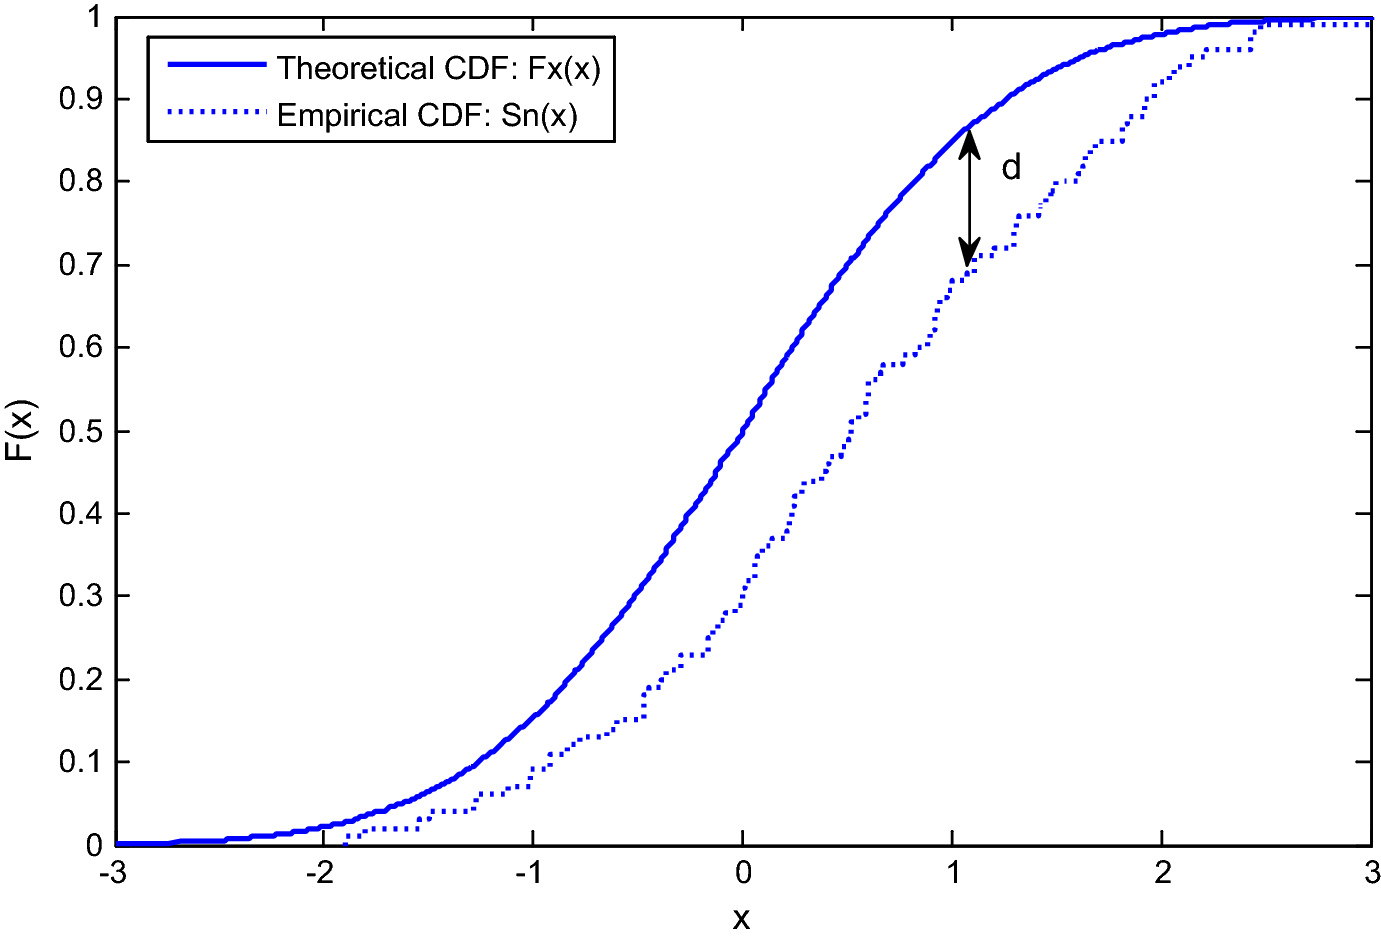
\includegraphics[scale=.75]{ks_test.png}\\
  \caption{KS Distance}
\end{figure}

Having established a lower bound for our power-law behavior, we can now calculate a scaling parameter $\alpha$, which turns out to be a  maximum likelihood estimation (MLE)\footnote[8]{A maximum likelihood estimator is a technique to generate a parameter that has the highest probability of being the actual parameter, in this case the actual $\alpha$ that when used in Eq.(11) describes a given curve.  Its derivation is beyond the scope of this paper.  The interested reader may consult Clauset (2009) or any formal text on probability and statistical inference for more information, e.g., Hogg and Tanis (1983).}, given by the formula:

\begin{align}
\alpha = 1 +\left[ \sum_{i=1}^{n}ln\frac{x_i}{x_{min}}\right]^{-1}
\end{align}

With these parameters, we can perform a goodness of fit test for our best fit model, in this case the power law for which we have calculated an $\alpha$ in Eq.(13). Here the criterion for best fit is how well a given frequency distribution fits a power law distribution. We calculate the KS statistic between our empirical data and our best fit model.  We then create many synthetic data sets by sampling a discrete power-law distribution equivalent to our best fit. Synthetic data sets (SDS) are computationally generated artifacts for use in the best fit process. 
Think of the process of generating synthetic data as the bootstrapping necessary to estimate the p-value.  Since the true distribution of the KS statistic is not known, the p-value cannot be calculated exactly. Under the assumption of the null hypothesis, we can sample from our assumed null distribution and therefore estimate the p-value.

An SDS is generated by uniformly sampling a continuous interval, [0,1]  and transforming the results so that they lie on a discrete power law distribution (Clauset, \emph{et al.}, 2009, Appendix D).  We then fit each synthetic data set to its own power-law model, by calculating its KS statistic relative to its best fit model. Figure 4 illustrates this process.  

In this study, a p-value is the number of data sets with a KS distance greater than its best fit model divided by the number of synthetic data sets.   For example, one would expect the Brown corpus of written text, the first million word corpus of English (Jurafsky and Martin, 2009), to be Zipfian.  In fact, we find that it has a p-value of 0.37.  Clauset \emph{et al} (2009) empirically determined that a p-value $\geq$ .1 is significant evidence that the data is drawn from a power law distribution.  We can now state our hypothesis with precision:

\begin{itemize}
\item $H^0$: The data is drawn from a power-law distribution
\item $H^1$: The data is not drawn from a power-law distribution
\end{itemize}

The number of synthetic data sets needed, of course, will affect the accuracy of the p-value computation, where the accuracy is expressed as the p-value plus or minus some $\epsilon$. The empirical relation between N, the number of synthetic data sets and  $\epsilon$ is given in: 

\begin{align}
N = \frac{1}{4{\epsilon}^2}
\end{align}

For our work, we set N to 5000 data sets, giving us $$\epsilon  = 7.07*10^{-3}$$ This guarantees a p-value with an uncertainty less than  $\pm0.01$. We use the more conservative $p \geq 0.10$ as a cutoff for power-law behavior. P-values less than 0.1 are considered evidence against power-law behavior.  

At this point in the analysis, we could compare our proposed power law distribution with other possible distributions.  This is unnecessary for very low p-values, since a low p-value rules out a power law distribution.  For larger p-values though, we could analyze the goodness of fit for other distributions in order to determine if a power-law is the best among them.  These other distributions, such as Poisson and log-normal occur frequently in nature and are possible candidates.  For example, mutation counts in genomes (Balin \emph{et al.} 2010) and income distribution of low-middle income groups (Clementi \emph{et al.} 2005) can be described by Poisson and log-normal distributions, respectively.  To compare power-law distributions to other distributions, we used a likelihood ratio test as proposed by Vuong (1989), as cited in Clauset, \emph{et al.}, (2009), a topic we turn to in the next section.


\subsection{Methods: Likelihood Ratio Test}

To determine which of two hypothetical distributions is more likely,  we  calculate the product of the probabilities of each data point for each data set and choose the highest number.  The individual probabilities come from the probability density function itself, Eq.(11), for example.  The result, since it is a product of many small decimal fractions, is likely to be very small. We take the logarithm of this small decimal fraction for ease and clarity of exposition.   In addition to the likelihood ratio, we also derive a p-value to indicate the significance of the ratio test.  A small p-value indicates an insignificant result.  Given probability density functions $p_{1}(x)$ and $p_{2}(x)$,  let $L_1$ be the likelihood of $p_1$ and $L_2$ be the likelihood of $p_2$ over all instances such that:

\begin{align*}
L_{1} = \prod_{i=1}^{n} p_{1}(x_{i}) \text{\quad and \quad} & L_{2} = \prod_{i=1}^{n} p_{2}(x_{i})
\end{align*}

Then \emph{R} is the ratio of $L_{1}$ and $L_{2}$:
\begin{align*}
R = \frac{L_{1}}{L_{2}} = \prod_{i=1}^{n}\frac{p_{1}(x_i)}{p_{2}(x_i)}
\end{align*}

Taking the log, we get the log-likelihood ratio:
\begin{align*}
\widetilde{R} = \sum_{i=1}^{n}\left[\ln p_{1}(x_i)-\ln p_{2}(x_i)\right]
\end{align*}

Since each sample $x_{i}$ is independent of other samples, then by the central limit theorem, the difference of our log-likelihoods will tend toward a normal distribution for large $n$.  From this, we can derive a p-value for the probability that the log-likelihood ratio would be as large or larger than our observed value. Given the normal distribution between the log-likelihoods, we can calculate the p-value using the complementary error function (\emph{erf}) of the resultant normal distribution, 

\begin{align*}
p = |\textrm{\emph{erf}}(\frac{\widetilde{R}}{\sqrt{2n\sigma}})|
\end{align*}

\noindent where $n$ is the number of instances and $\sigma$ the standard deviation.  The error function, \emph{erf}, from the R statistical package, indicates the probability of error between $\pm{R}$ by calculating the area under the normal distribution curve.   It is worth noting that a small p-value where p $\leq$0.10 would imply a statistically insignificant result. Thus, our likelihood test can tell us which distribution is favored, how strongly it is favored, and whether the difference is significant.

\section{Results}

We begin with the goodness of fit test, the results for which are found in Table 4.  Initially, we can observe that under a conservative p-value of p $\geq$ 0.10 unigrams (words) in most of the corpora under examination are consistent with a Zipfian distribution. The exceptions were the Buckeye and ATIS corpora. If we used the more liberal cutoff of p $\leq$ 0.05, then only the ATIS corpus is disqualified.

The bigram case seems to be strongly non-Zipfian, with only the Czech bigrams giving evidence for power-law behavior. The trigrams are a mixed group, with the Buckeye, Santa Barbara and ATIS corpora qualifying. The quadgrams, like the bigrams, seem safely non-Zipfian, with only one corpus giving indication of power-law behavior. The combined n-grams case is mixed.  Given the strength of the results for unigrams and the mixed results for multiword sequences, the initial results cast doubt on the possibility of multi-word sequences being Zipfian.  These results deviate sharply from those reported in Ha, \emph{et al.} who, through visual inspection, confirm the findings of Herbert Simon and others that Zipf's law "did not hold for $r > 5000$" (2002 p. 2).  Still, the major contribution of Ha \emph{et al.} is the rather remarkable finding that the collection of all gram sizes from the Wall Street Journal corpus with several million words, at least through visual inspection, appears Zipfian.  As Table 4 indicates, our all-gram experiment on the Brown corpus indicates that not only is Zipfianniness not increased by putting all grams into a single file, but doing so renders it decidedly un-Zipfian.


\begin{table}[H]
\caption{p-values by corpus}
\begin{center}
\begin{tabular}{ |l|l|l|l|l|l| } 
\hline
 Corpus & Unigram & Bigram & Trigram & Quadgram & All Gram\\ [0.5ex] 
 \hline
 Buckeye & 0.06 & 0.00 & 0.35 & 0.00 & 0.00 \\ 
 MiCase & 0.15 & 0.00 & 0.00 & 0.02 & 0.07\\
 Fisher & 0.78 & 0.00 & 0.00 & 0.03 & 0.00 \\ 
 ATIS & 0.00 & 0.00 & 0.31 & 0.35 & 0.00 \\
 Santa Barbara & 0.58 & 0.00 & 0.62 & 0.00 & 0.45 \\
 Czech Telephone & 0.15 & 0.76 & 0.00 & 0.00 & 0.47 \\
 Brown & 0.37 & 0.02 & 0.02 & 0.00 & 0.00 \\ 
 \hline
\end{tabular}
\end{center}
\end{table}

The frequency counts of these distributions from peak ($x_{max}$) to cutoff ($x_{min}$) are shown in Table 5.  The lower bound, $x_{min}$, is generated by the goodness of fit test as described above.  Given the substantial difference between each $x_{min}$ and $x_{max}$ over all corpora as shown in Table 5, the the great bulk of the distributions lie within the peaks and cutoffs and are being considered in the power law fit computations.


\begin{table}[H]
\caption{$x_{min}$ and $x_{max}$ by Corpus}
\begin{center}
\begin{tabular}{| *{11}{l|} }
    \hline
$x_{max}$, $x_{min}$    & \multicolumn{2}{l|}{Unigram}
            & \multicolumn{2}{l|}{Bigram}
                    & \multicolumn{2}{l|}{Trigram}
                            & \multicolumn{2}{l|}{Quadgram} 
                            & \multicolumn{2}{l|}{All Gram}\\
    \hline
Buckeye   &   11962  &   5  & 1383 & 2&   559  &   3  &   94  &   1  &   11962  &   5  \\
    \hline
MiCase   &   74644  &   38  &   7404  &   4  &   1451  &   4  &   250  &   4 & 74644 & 11  \\
    \hline
Fisher   &  322401 & 151 & 101464 & 3 & 17536 & 3 & 3393 & 5 & 322401 & 16\\
    \hline
ATIS   &  8098     &    1   &   2127    &   1    &      1348 &  7     &     500  &      4 & 8098 & 3 \\
    \hline
Santa Barbara   &  8075     &   7    &  1456     &      3 & 314& 3&  46      & 1      & 8075      &      9 \\    \hline
Czech Telephone   &   6732    &     8  &    1216   &    5   &  776     &     1  & 446       & 1     & 6732 & 16  \\
    \hline
Brown & 69971 & 53 & 9740 & 3 & 404 & 4 & 111 & 1 & 69971 & 6 \\
    \hline
\end{tabular}
\end{center}
\end{table}

All of the corpora, with the exception of Buckeye and ATIS are Zipfian with respect to words by our conservative definition of $p \geq{0.1}$ (though only ATIS is non-Zipfian by our more liberal cutoff of 0.05).  Might these two be described by another distribution?   Recall, that for every log-likelihood ratio test, there is a corresponding p-value.  

Table 6 shows the comparison of the power law distribution to other distributions.   A p-value $\geq$ 0.10 indicates a significant comparison.  A sufficiently large negative \emph{R} value favors the alternative distribution, whereas a small negative or positive value favors the power law. The take-away is that both Buckeye and ATIS appear to be described by a log-normal distribution.  There is a muddier observation to make, however.   Though Fisher is Zipfian by the goodness of fit test (Table 4), it could be log-normal by the ratio test (Table 6). At this point, we have to ask ourselves if there is a linguistic reason why we should prefer one over the other.  We can always come up with a new distribution that fits a data set better than some alternative.  The danger is over-parameterizing.  The linguistic reason is that language samples, including speech, it seems, form power law distributions.  For now, we cannot reject the claim that, with respect to Fisher, both log-normal and power law appear to fit the phenomenon.  

We note that Brown, a written corpus, appears less Zipfian than two of the spoken corpora, Fisher and Santa Barbara. Nevertheless, unless p-values differ by, say, an order of magnitude, as they do not in this case, we caution against asserting that one corpus is more or less Zipian than another.  

Finally, none of the corpora are either Poisson or exponential. In fact, when they deviate from the power law distribution, they deviate towards log-normal.  This is not surprising given that with respect to tail decay--large x-values becoming rare--power law and log-normal distributions are similar as are Poisson and exponential distributions.  
\begin{table}[H]
\caption{Comparison Test by Corpus}
\begin{center}

\begin{tabular}{| *{7}{l|} }
    \hline
p, R& \multicolumn{2}{l|}{Log-normal}
            & \multicolumn{2}{l|}{Poisson}
                    & \multicolumn{2}{l|}{Exponential}\\
    \hline
Buckeye  & 0.06 & -1.82 & 0.00 & 6.85 & 0.00 & 7.80 \\
    \hline
MiCase & 0.50 & 0.67 & 0.00 & 6.48 & 0.00 & 7.11  \\
    \hline
Fisher   & 0.06 & -1.88 & 0.00 & 6.66 & 0.00 & 7.48\\
    \hline
ATIS   & 0.00 & -5.62 & 0.00 & 7.03 & 0.00 & 8.11\\
    \hline
Santa Barbara  & 0.43 & -0.79 & 0.00 & 6.91 & 0.00 & 13.67  \\
    \hline
Czech Telephone & 0.36 & -0.91 & 0.00 & 5.06 & 0.00 & 9.14   \\
    \hline
Brown & 0.21 & 1.24 & 0.00 & 3.87 & 0.00 & 4.42 \\
    \hline
\end{tabular}
\end{center}
\end{table}

\section{Conclusion and Future Research}

In this paper we have:  

\begin{itemize}
\item Shown (Section 2) that Zipf's Law and the Zipfian distribution (Zipf, 1949) is a special case of the more general power law distribution.
\item Argued (Section 3) that spontaneous spoken language is sufficiently different from written language to warrant an investigation into whether it can be characterized by a power law distribution. 
\item Presented (Section 4) a goodness of fit test based on the Kolmogorov-Smirnov (KS) statistic and maximum likelihood estimation (MLE) that is a more sophisticated technique for judging power-law fit than what is conventionally found in the literature on Zipf's Law.
\item Presented (Section 4) a technique based on the complementary error function for normal distributions that can be used to judge whether a corpus, failing the goodness of fit test for the power law, can be better described by another distribution.
\item Found (Section 5) that all five tested corpora of what can reasonably be called \emph{spontaneous spoken language (SSL)} follow a power-law distribution, four of them strongly so.  Though we believe that the data and analyses provided in this study warrant the tentative conclusion that spontaneous spoken speech follows a power law distribution, the presence of Buckeye at the lower end of acceptability requires further investigation. 
\end{itemize}

One  might  ask  why  anyone  should  care  about  word  distributions.   We  believe  the  answer to this question is the same answer that mathematicians and scientists have been offering for decades, if not centuries.  Looking for regularities in any natural phenomenon–including language–is interesting and important,  because knowing is better than not knowing;  but mostly, this is what we humans have been doing fairly consistently since the beginnings of the scientific revolution in the early modern period. Zipf spent his career puzzling over word frequencies, and, as it happens, he was quite prescient in doing so.  One can hardly read him without thinking about the importance of frequency in all its forms to usage-based investigations of language.   Joan Bybee, in particular, has foregrounded frequency--in phonology, among types and tokens, in grammaticalization and language change generally--as a crucial aspect of language (Bybee, 2001, 2005, 2010).  In a combination review of Bybee's most recent book (\emph{Language, Usage and Cognition}, 2010) and introduction to usage-based linguistics, Holger Diessel argues that
\begin{quote}
... frequency itself is not a cognitive phenomenon; the term simply denotes the occurrence of objects or events in a particular domain or time frame. But frequency of occurrence is an important factor in almost all cognitive processes that are involved in usage and development: it underlies the emergence of exemplar-based categories (Ch. 2); it influences analogy and pragmatic inference (Chs. 4 and 10; and it has a major impact on grammaticalization and other aspects of diachronic change (especially Chs. 3 and 6).  Diessel (2011, p. 833).
\end{quote}
Might the use of new statistical techniques of the kind explored in this paper contribute to theoretical language study beyond power law behavior?  We think so.  Perhaps it is only a matter of linguists having easy access to the right tools, tools built for linguists instead of computer and data scientists.  We plan to package the tools described in Section 4.1 as the \emph{Zipfian Tool Kit} and make them available on GitHub.

But the value of word distribution investigation do not end with the theoretical.  Potential applications abound.  Zipf's own preliminary examination of the speech of people diagnosed with schizophrenia (Zipf, 1949), along with our finding that all five SSL corpora follow a power law distribution, point to at least one. New and complex statistical techniques, including machine-learning, when applied to the larger speech corpora now available may be useful in the diagnoses of those conditions that can include disordered speech.  Van Egmond \emph{et al} (2015) have examined non-fluent aphasia, citing Clauset, but with a tiny sample size ($n = 4$).  Hernandez-Fernandez and Dieguez-Vilde (2013), find that the progression of Alzheimer's can be tracked using Zipf's Law, also using a small sample ($n = 20$), but through a log-log plat and linear regression.  At this point, we have made a preliminary examination of some of the corpora available through TalkBank (talkbank.org), specifically AphasiaBank (MacWhinney, \emph{et al.}, 2011) and DementiaBank (Becker \emph{et al.}, 1994). We hope to report our results in the near future.

Finally, we should mention that we are part of a growing group of researchers interested in using computational techniques to explore regularities in spoken language (DARCLE, 2020).  Very large-n corpora of children's speech already exist and are being continuously augmented.  HomeBank, part of the TalkBank project at Carnegie-Mellon, is an example (VanDam, \emph{et al.}, 2016). We have used thousands of hours of recordings to investigate child-directed speech in the home (De Palma \& VanDam, 2017; VanDam \emph{et al.}, 2015)  Very large corpora bring, along with enormous possibilities, issues of their own, yet to be entirely resolved (VanDam \& De Palma, 2019).  Zipf was onto something big in 1929. He could not have imagined what would become available for language study less then a century later.  Indeed, researchers \emph{circa} 1975 might not have believed it either.  The possibilities, if not endless, sometimes seem so.    


\begin{thebibliography}{50}

\bibitem{Bloomberg}
\emph{Bloomberg Billionaire's Index} (2020, May 7). \\
\url{https://www.bloomberg.com/billionaires.} 

\bibitem{Bybee0}
Bybee, J. (2001).  \emph{Phonology and language use}. Cambridge Studies in Linguistics 94. Cambridge, UK: Cambridge University Press.

\bibitem{Bybee0}
Bybee, J. (2006).  From Usage to Grammar: The Mind's Response to Repetition. \emph{Language}, 82(4),711-733.

\bibitem{Bybee2}
Bybee, J. (2010).  \emph{Language, usage, and cognition}. Cambridge, UK: Cambridge University Press.

\bibitem{Balin}
Balin, S., Cascalho, M. (2010). The rate of mutation of a single gene. \emph{Nucleic acids research}, 38(5), 1575-1582.

%\bibitem{Baayen}
Baayen, R. Harald (2001).  \emph{Word frequency distributions}. Dordrecht: Kluwer Academic Publishers.

\bibitem{Bybee0}
Bybee, J. (2001).  \emph{Phonology and language use}. Cambridge Studies in Linguistics 94. Cambridge, UK: Cambridge University Press.

\bibitem{Bybee0}
Bybee, J. (2006).  From Usage to Grammar: The Mind's Response to Repetition. \emph{Language}, 82(4),711-733.

\bibitem{Bybee2}
Bybee, J. (2010).  \emph{Language, usage, and cognition}. Cambridge, UK: Cambridge University Press.

\bibitem{Becker}
Becker, J. T., Boller, F., Lopez, O. L., Saxton, J., \& McGonigle, K. L. (1994). The natural history of Alzheimer's disease: description of study cohort and accuracy of diagnosis. \emph{Archives of neurology}, 51(6), 585-594.

\bibitem{Clementi}
Clementi F., Gallegati M. (2005) Pareto’s law of income distribution: evidence for Germany, the United Kingdom, and the United States. In: Chatterjee A., Yarlagadda S., Chakrabarti B.K. (eds) \emph{Econophysics of wealth distributions. New economic windows}. Milano: Springer.

\bibitem{Fisher}
Cieri, C., Miller, D., Walker, K. (2004, May). \emph{The Fisher Corpus: a resource for the next Generations of speech-to-text}. \emph{Proceedings of the fourth international on languages resources and evaluation}, 4, 69-71. 

\bibitem{Clauset}
Clauset, A., Shalizi, C. R., Newman, M. E. J. (2009). Power-law distributions in empirical data. \emph{SIAM review}, 51(4), 661–703. doi:10.1137/070710111.

\bibitem{ATIS}
Dahl, Deborah A., et al. (1995) \emph{TIS3 test tata LDC95S26}. Philadelphia: Linguistic Data Consortium.

\bibitem{DARCLE}
DARCLE: Daylong audio recordings of children's linguistic environments.
\url{darcle.org}.

\bibitem{DePalma}
De Palma, P., VanDam, M. (2017).  Using automatic speech processing to analyze fundamental frequency of child-directed speech stored in a very large audio corpus. \emph{Proceedings of the joint 17th world congress of international fuzzy systems association and 9th international conference on soft computing and intelligent systems}. Otsu, Japan, June 27-30, 2017.

\bibitem{Diessel}
Diessel, H. (2011). Language, usage, and cognition (review). \emph{Language}, 87(4),830-844.

\bibitem{SantaBarbara}
Du Bois, J., Chafe, W.,  Meyer, C., Thompson, S., Englebretson, R., Martey, N. (2000-2005). \emph{Santa Barbara corpus of spoken American English, Parts 1-4}. Philadelphia: Linguistic Data Consortium.

\bibitem{fedorowicz}
Fedorowicz, J. (1982). The theoretical foundation of Zipf's law and its application to the bibliographic database environment. \emph{Journal of the American society for information science}. September, 285-293.

\bibitem{Ferrer i Cancho}
Ferrer i Cancho, R. (2005). Zipf's Law from a communicative phase transition.  \emph{The European physical journal B}, 47, 449-457. doi: 10.1140/epjb/e2005-00340-y.

\bibitem{Brown}
Francis, W. N., Kucera, H. (1979). \emph{Brown corpus manual: manual of information to accompany a standard corpus of present-day edited American English for use with digital computers}. Providence: Brown University.

\bibitem{Gutenberg}
\emph{Project Gutenberg} (2020, June 17). \\
\url{https://www.gutenberg.org}.

\bibitem{Greenhough}
Greenhough, John, and I. G. Main. (2008). A Poisson model for earthquake frequency uncertainties in seismic hazard analysis. \emph{Geophysical research letters}, 35(19).

\bibitem{Gross}
Gros, C., Kaczor, G., Marković, D. (2012). Neuropsychological constraints to human data production on a global scale. \emph{The European physical journal B}. 85(1),28.

\bibitem{ha}
Ha, L. Q., Sicilia-Garcia, E. I., Ming, J., Smith, F. J. (2002, August). Extension of Zipf's law to words and phrases. \emph{Proceedings of the 19th international conference on computational linguistics}. 1,1-6. 

\bibitem{Hanley}
Hanley, M.L. (1962). \emph{Word index to James Joyce's Ulysses}. Madison: University of Wisconsin Press. (Original work published 1937).

\bibitem{Hernandez}
Hernandez-Fernandez, A., Dieguez-Vide, F. (2013). La ley de Zipf y la detección de la evolución verbal en la enfermedad de Alzheimer. \emph{Anuario de sicología}, 43(1), 67-82.

\bibitem{Jurafsky}
Jurafsky, D., Martin, J. (2009). \emph{Speech and Language Processing}. Upper Saddle River, NJ: Pearson.

\bibitem{Hogg}
Hogg, R., Tanis, E. (1983). \emph{Probability and statistical inference}, NY: Macmillan Publishing Company.

\bibitem{CzechTelephone}
Korvas, M., Plátek, O., Dušek, O., Žilka, L., Jurčíček, F. (2014, May). Free English and Czech telephone speech corpus shared under the CC-BY-SA 3.0 license. \emph{Proceedings of the ninth international conference on language resources and evaluation}. 4423-4428.

\bibitem{MacWhinney}
MacWhinney, B., Fromm, D., Forbes, M. \& Holland, A. (2011). AphasiaBank: methods for studying discourse. \emph{Aphasiology},25,1286-1307.

%bibitem{Miller}
Miller, J., Weinert, R. (1998).  \emph{Spontaneous spoken language: syntax and discourse}, Oxford: Oxford University Press. 

\bibitem{Newman}
Newman, M. E. J. (2005). Power laws, Pareto distributions and Zipf's law.  \emph{Contemporary physics}, 46(5), 323-351.

\bibitem{NLTK}
\emph{NLTK.tokenize Package} (2020, May 17).  \\ 
\url{https://www.nltk.org/api/nltk.tokenize.html?highlight=word_tokenize#nltk.tokenize.word_tokenize}.

\bibitem{ong}
Ong, W. 1958.  \emph{Ramus, method, and the decay of dialogue: from the art of discourse to the art of reason}, Cambridge: Harvard University Press.

\bibitem{Parry}
Parry, M. (1971).  \emph{The Making of Homeric Verse}, Oxford: Oxford University Press. (Originally published from 1928 to 1936).

\bibitem{Buckeye}
Pitt, M.A., Dilley, L., Johnson, K., Kiesling, S., Raymond, W., Hume, E. and Fosler-Lussier, E. (2007) \emph{Buckeye Corpus of Conversational Speech}.  2nd release. www.buckeyecorpus.osu, Columbus, OH: Department of Psychology, Ohio State University (Distributor).

\bibitem{Ridley}
Ridley, D., Gonzales, E. (1994). Zipf's law extended to small samples of adult speech.  \emph{Perceptual and motor skills}, 79, 153-154. 

\bibitem{MICASE}
Simpson, R. C., S. L. Briggs, J. Ovens, and J. M. Swales. (2002). \emph{The Michigan corpus of academic spoken english}. Ann Arbor, MI: The Regents of the University of Michigan.

\bibitem{Rojas-Lima}
Rojas-Lima, J., Hernandez-Aguilar, C., Simon, L., Cruz-orea, A. (2019). Kolmogorov–Smirnov test for statistical characterization of photopyroelectric signals obtained from maize seeds. \emph{International journal for themophysics}, 40(4).

\bibitem{Tomasello}
Tomasello, M. (2003).  \emph{The New psychology of language, Volume 2}. Mahwah, NJ: Lawrence Erlbaum and Associates. 

\bibitem{van Egmond}
Van Egmond, M., Van Ewijk, L., Avrutin, S. (2015). Zipf’s law in Non-fluent aphasia. Journal of quantitative linguistics, 22(3), 233-249, DOI:
10.1080/09296174.2015.1037158

\bibitem{vanDam0}
VanDam, M.  De Palma, P., Strong, W., Kelly, E. (2015). Child-Directed Speech of Fathers. Poster, 89th Annual Meeting of the Linguistic Society of America, Portland, OR, Jan. 2015.

\bibitem{VanDam1}
VanDam, M., Warlaumont, A. Bergelson, E., Cristia, A., Soderstrom, M., De Palma, P., 
Mac Whinney, B.  (2016).  HomeBank: an online repository of daylongy child-centered audio recordings.  \emph{Seminars in speech and language}.  37(02), 128-142.

\bibitem{VanDam2}
VanDam, M., De Palma, P. (2019).  A modular, extensible approach to massive ecologically-valid behavioral data.  \emph{Behavioral research methods}, 51(4), 1754-1765. doi: 10.3758/s13428-018-1167-8. Springer in cooperation with the Psychonomic Society. 

\bibitem{Vuong}
Vuong, Q. H. (1989). Likelihood ratio tests for model selection and non-nested hypotheses. \emph{Econometrica: journal of the econometric society}, 307-333.

\bibitem{Zipf0}
Zipf, G. K. (1949). \emph{Human behavior and the principle of Least effort: An introduction to human ecology}. Cambridge: Addison-Wesley.

\bibitem{Zipf1}
Zipf, G. K. (1932). \emph{The psycho-biology of language}. Cambridge: Harvard University Press. 

\bibitem{Zipf2}
Zipf, G. K. (1929). Relative frequency as a determinant of phonetic change. \emph{Harvard Studies in Classical Philology}, 40, 1-95.

\end{thebibliography}
\end{document}






















